%%%%%%%%%%%%%%%%%%%%%%% file template.tex %%%%%%%%%%%%%%%%%%%%%%%%%
%
% This is a template file for Acta Informatica
%
% Copy it to a new file with a new name and use it as the basis
% for your article
%
%%%%%%%%%%%%%%%%%%%%%%%% Springer-Verlag %%%%%%%%%%%%%%%%%%%%%%%%%%
%
% First comes an example EPS file -- just ignore it and
% proceed on the \documentclass line
\begin{filecontents*}{example.eps}
%!PS-Adobe-3.0 EPSF-3.0
%%BoundingBox: 19 19 221 221
%%CreationDate: Mon Sep 29 1997
%%Creator: programmed by hand (JK)
%%EndComments
gsave
newpath
  20 20 moveto
  20 220 lineto
  220 220 lineto
  220 20 lineto
closepath
2 setlinewidth
gsave
  .4 setgray fill
grestore
stroke
grestore
\end{filecontents*}
%
\documentclass[actinf,referee]{svjour}
% Remove option referee for final version
%
% Remove any % below to load the required packages
%\usepackage{latexsym}
\usepackage{graphics}
% etc
%
\begin{document}
%
\title{Insert your title here}
\subtitle{Do you have a subtitle?\\ If so, write it here}
\author{First author\inst{1} \and Second author\inst{2}% etc
% \thanks is optional - remove next line if not needed
\thanks{\emph{Present address:} Insert the address here if needed}%
}                     % Do not remove
%
\offprints{}          % Insert a name or remove this line
%
\institute{Insert the first address here \and the second here}
%
\date{Received: date / Revised version: date}
% The correct dates will be entered by the editor
%
\maketitle
%
\begin{abstract}
Insert your abstract here.
\end{abstract}
%
\section{Introduction}
\label{intro}
Your text comes here. Separate text sections with
\section{Section title}
\label{sec:1}
and \cite{RefJ}
\subsection{Subsection title}
\label{sec:2}
as required. Don't forget to give each section
and subsection a unique label (see Sect.~\ref{sec:1}).
%
% For one-column wide figures use
\begin{figure}
% Use the relevant command for your figure-insertion program
% to insert the figure file.
% For example, with the option graphics use
\resizebox{0.75\textwidth}{!}{%
  \includegraphics{example.eps}
}
% If not, use
%\vspace{5cm}       % Give the correct figure height in cm
\caption{Please write your figure caption here}
\label{fig:1}       % Give a unique label
\end{figure}
%
% For two-column wide figures use
\begin{figure*}
% Use the relevant command for your figure-insertion program
% to insert the figure file. See example above.
% If not, use
\vspace*{5cm}       % Give the correct figure height in cm
\caption{Please write your figure caption here}
\label{fig:2}       % Give a unique label
\end{figure*}
%
% For tables use
\begin{table}
\caption{Please write your table caption here}
\label{tab:1}       % Give a unique label
% For LaTeX tables use
\begin{tabular}{lll}
\hline\noalign{\smallskip}
first & second & third  \\
\noalign{\smallskip}\hline\noalign{\smallskip}
number & number & number \\
number & number & number \\
\noalign{\smallskip}\hline
\end{tabular}
% Or use
\vspace*{5cm}  % with the correct table height
\end{table}
%
% BibTeX users please use
% \bibliographystyle{}
% \bibliography{}
%
% Non-BibTeX users please use
\begin{thebibliography}{}
%
% and use \bibitem to create references.
%
\bibitem{RefJ}
% Format for Journal Reference
Author, Journal \textbf{Volume,} (year) page numbers.
% Format for books
\bibitem{RefB}
Author, \textit{Book title} (Publisher, place year) page numbers
% etc
\end{thebibliography}


\end{document}

% end of file template.tex

